\chapter{Physics-based Human Neck Modeling and Simulation}
\label{ch:vriphys}
In deformable character animation, the skin deformation of the neck is important to reproduce believable facial animation, and the neck also plays an important role in supporting the head in balance while generating the controlled head movements that are essential to so many aspects of human behavior. However, neck animation is largely overlooked both in computer graphics and animation due to the complexity of the cervical anatomy.

This chapter presents a physical human neck model based on biomechanical modeling. Relevant anatomical structures available in a 3D model of human musculoskeletal system are modeled as deformable or linked rigid bodies. We couple the soft-hard bodies using soft constraints via elastic springs and form a Lagrangian dynamic system. The simulation of dynamic skin deformation is achieved by automatically binding the vertices to underlying bodies in an anatomical manner. Experimental results are provided and show high level of realism our model offers, and the simulation runs at interactive rates on a modern computer.

%-------------------------------------------------------------------------
\section{Introduction}
\label{sec:intro}
Characters should be capable of expressing their physical states and emotional expressions convincingly in a 3D virtual environment. To achieve that, many efforts are afforded to increase the realism of important aspects, e.g. facial animation~\cite{Sifakis:2005:facial,Fratarcangeli:2005:physically,Zhang:2004:NPM}, tear simulation~\cite{van:2009:real}, skinning of a skeletally-based deformable body~\cite{Kavan:2007:SDQ}, and breathing simulation~\cite{Zordan:2004:breathe}.

As an aspect of non-verbal communication in character animation, neck animation should be considered as of importance. On the one hand, we could be inclined to perceive the displeasing distortion of the neck skin in the facial animation. On the other hand neck plays an important role in supporting the head in balance while generating the controlled head movements that are essential to so many aspects of human behavior.

However, to our knowledge the neck animation has been overlooked both in computer graphics and animation despite~\cite{Lee:2006:HUB} and ~\cite{vasavada:1998:influence}. These latter have investigated human neck simulations where only motions generated kinematically and biomechanically are visualized without much visual richness. Those less detailed models generally are not suitable for skin deformation and therefore more detailed models accounting for the deformation of underlying soft tissues were proposed ~\cite{Lee:2009:CBM} for the upper human body and~\cite{Assassi:2012:dynamic} for the lower body. Nonetheless, they are not applicable in interactive character animation due to the highly computational cost.

Current approaches rely on approximations by using techniques such as skeletally-based skinning~\cite{Kavan:2007:SDQ} for real-time neck animation. In general, they guarantee a degree of realism only from the graphical visualization and therefore lack physical accuracy, or like~\cite{Lewis:2000:PSD} often requires considerable manual work. In the case the propagation of muscle motion to the skin layer is visible, modeling of muscle deformation has been investigated based on dense motion capture data~\cite{Park:2008:DMS,Neumann:2013:muscles}. Nevertheless, accounting for the physical or biomechanical facts, learning a model of muscle deformation only from captured skin motion cannot guarantee the accuracy of simulating the muscle dynamics. Attempts to alleviate this shortcoming have been given by~\cite{Sifakis:2005:facial} which learned the facial muscle functions from skin motion based on a pre-defined physical face model, and~\cite{Tan:2012:SBL} decided muscle activations in a fibre-driven soft body simulator from prescribed locomotion.
\begin{figure}
\centering
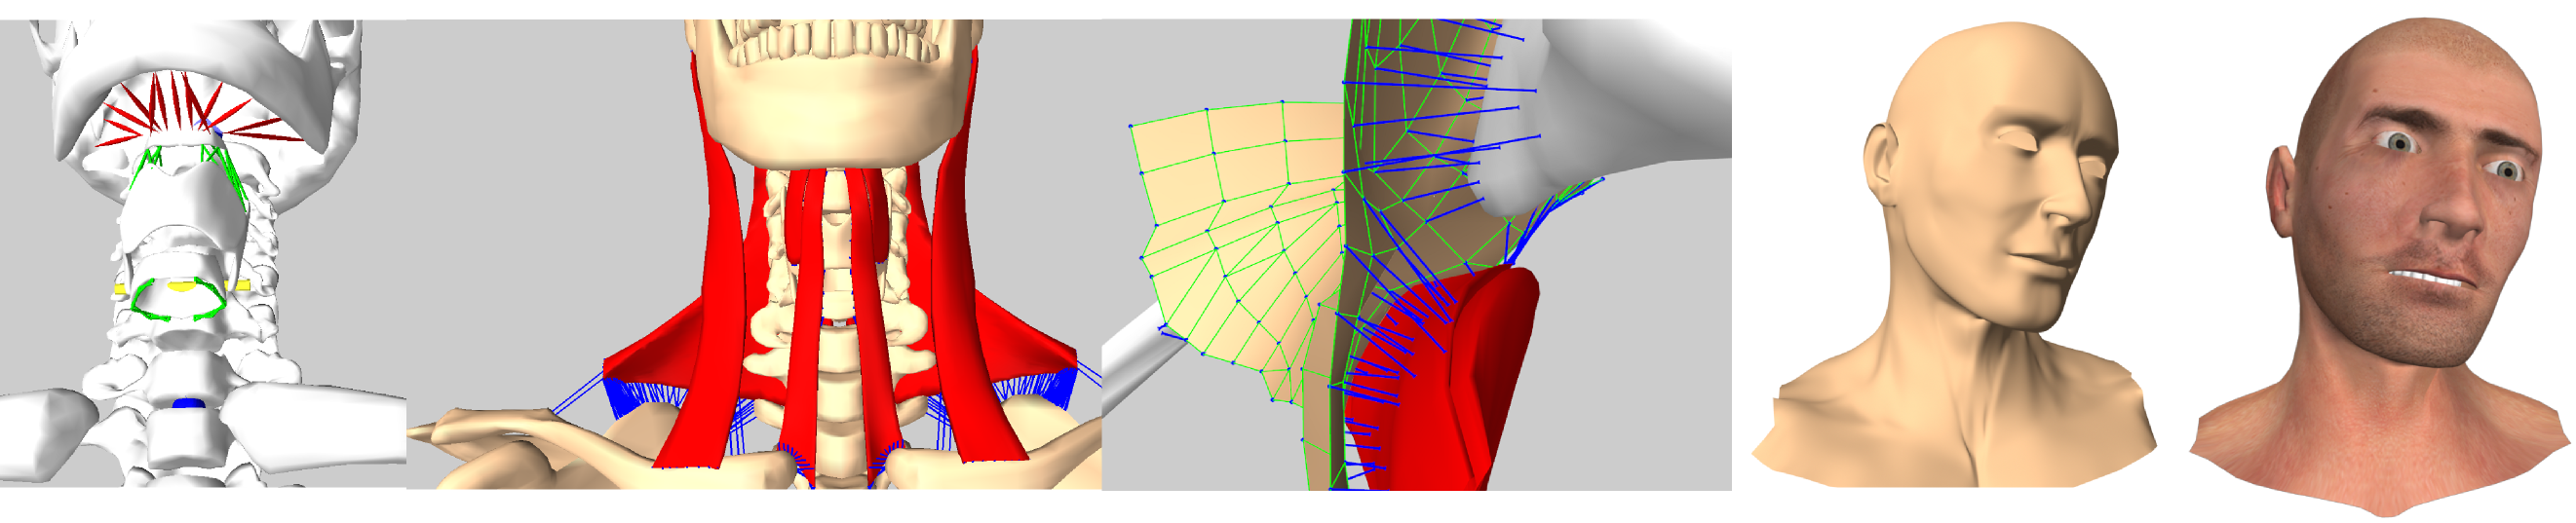
\includegraphics[width=\linewidth]{vriphys/pipline}
\caption{We simulate the biomechanics of the human neck and develop a physical skinning approach, and make use of the simulation in character animation. From left to right: skeleton, skeleton-driven muscle deformation, skinning, simulation, animation.}
\label{fig:teaser}
\end{figure}

In this chapter, we present a physical model for neck animation, whereas we directly investigate the biomechanics of the neck to solve the complexity of the cervical anatomy and then simulate the skin deformation based on simulated dynamics underneath (see Figure~\ref{fig:teaser}). The neck anatomy is from the Ultimate Human Model (UHM) data set~\cite{www:UHM} which includes a complete and accurate human musculoskeletal system. A novel approach is proposed to construct the musculoskeletal model that consists of deformable bodies and linked rigid bodies. In more details, we integrate the deformable bodies with the skeleton using a soft constraint concept and therefore the skeleton drives the muscle deformation. In order to use the simulated dynamics of the underlying system for skin deformation, we bind each skin vertex to one muscle or
bone by an elastic spring and this processing is automated. Thereby, the skin deforms when the skeleton moves. We simulate the neck at interactive rates because our modeling is based on linear elasticity (continuum) theory which is fast and easy to implement.

%-------------------------------------------------------------------------
\section{Previous Work}
\label{sec:previous}
We broadly classify the approaches proposed for character animation into the following categories. Our approach falls into the category of physically based methods.

\textbf{Geometric skinning}
For its simplicity and efficiency, skinning of skeletally deformable
body is extensively used in real-time character animation, especially the standard solution, linear blend skinning. Popularly, we bind each skin vertex to one or more joints. However, simple skinning will exhibit artifacts including skin collapsing effects though advanced alternatives, e.g.~\cite{Kavan:2007:SDQ} can remove some artifacts yet they still fall short of delivering natural skin deformation, and producing realistic musculature or dynamic effects.

\textbf{Example based techniques}
Such techniques beforehand provide a number of input examples,
and then synthesize the surface deformation using either direct interpolation between examples~\cite{Lewis:2000:PSD}, or more accurate yet more complex example interpolation~\cite{Rhee:2006:real}, or fitting the linear parameters to match the provided examples~\cite{Mohr:2003:BEA}. Generally, a level of realism only limited by the number of provided examples is offered. However, the generation of examples can be costly, requiring a lot of memory to store them and animator's labour~\cite{Lewis:2000:PSD}.

\textbf{Capturing real subjects}
These methods either exploit 3D scanning device to directly
capture the skin deformation~\cite{Allen:2003:SHB}, or complete the shape based on motion capture data~\cite{Park:2008:DMS,Anguelov:2005:SSC} of real people. Furthermore, muscle deformations also can be captured~\cite{Neumann:2013:muscles}. While these approaches are highly accurate, they require expensive hardware and are subject-specific.

\textbf{Physically based methods}
From the anatomical or physical view, it is logical to
animate characters by simulating the underlying musculoskeletal structures. Generally, the skeleton is modeled as an articulated multibody dynamic system~\cite{Lee:2006:HUB,Stavness:2011:CNM}, muscles, fat and skin tissue can be modeled by either finite element method~\cite{Capell:2002:ISD,Georgii:2010:SkeletalFEM,Muller:2002:SRD} or mass-spring system~\cite{Zordan:2004:breathe,Zhang:2004:NPM,Fratarcangeli:2005:physically}.

Assassi et al.~\cite{Assassi:2012:dynamic} developed a lower human body model consisting of finite element models, while Lee et al.~\cite{Lee:2009:CBM} the upper body. For visualization of the skin deformation, the former directly renders the model surface, whereas the latter embeds a high-resolution skin surface as the visualization geometry by means of barycentric interpolation of the surface nodes from the nodes of the tetrahedral simulation mesh.
%Physically-based methods
%are known to have high computational cost despite we obtain high level of realism including visible muscle motion.

%------------------------------------------------------------------------
\section{Modeling}
\label{modeling}
This section presents the neck mechanical system of which each major component is described hereafter, namely the skeleton, musculoskeletal structure, skin model and the numeric simulation.

%------------------------------------------------------------------------
\subsection{Skeletal Model}
\label{sec:skeletalmodel}
In character animation, generally head movements including flexion, extension, bending and rotation are generated directly by the configurations of joints in the neck spine instead of muscle actuation, and consequently result in deformation of the surrounding muscles. Consulting reference on the anatomy in the UHM data set, C1-C7 cervical vertebrae, hyoid, thyroid and cricoid are in the neck, and certain neck muscles span the bones including sternum, skull, clavicle scapula, costal cartilage and T1-T12 thoracic vertebrae. In our model, we will only model the muscles (see Section~\ref{sec:musclemodeling}) which are the most relevant to skin deformation, therefore only the bones which one or more of these muscles span are incorporated into our skeletal model.

We model the skeleton as an articulated, multi-body dynamic system where the bones are rigid bodies. As shown in Figure~\ref{fig:neckskeleton}, the skeletal model contains skull, hyoid, thyroid, cricoid, C1-C7, the base that is the combination of sternum, clavicle scapula, costal cartilage and T1-T3, and 3-DOF ball joints inserted between adjacent vertebrae, C1 and skull, base and C7 by carefully locating the pivot points as~\cite{Lee:2006:HUB}. Additionally, we adopt the structure from~\cite{Stavness:2011:CNM} which consists of a revolution joint constraining thyroid and cricoid using the same way as locating ball joints, crossed elastic springs (Eqn.~(\ref{eq:spring})) connecting cricoid and base, hyoid and thyroid, point-to-point muscle actuators (Section~\ref{sec:muscleactuationmodel}) coupling skull and hyoid.
\begin{figure}
\centering
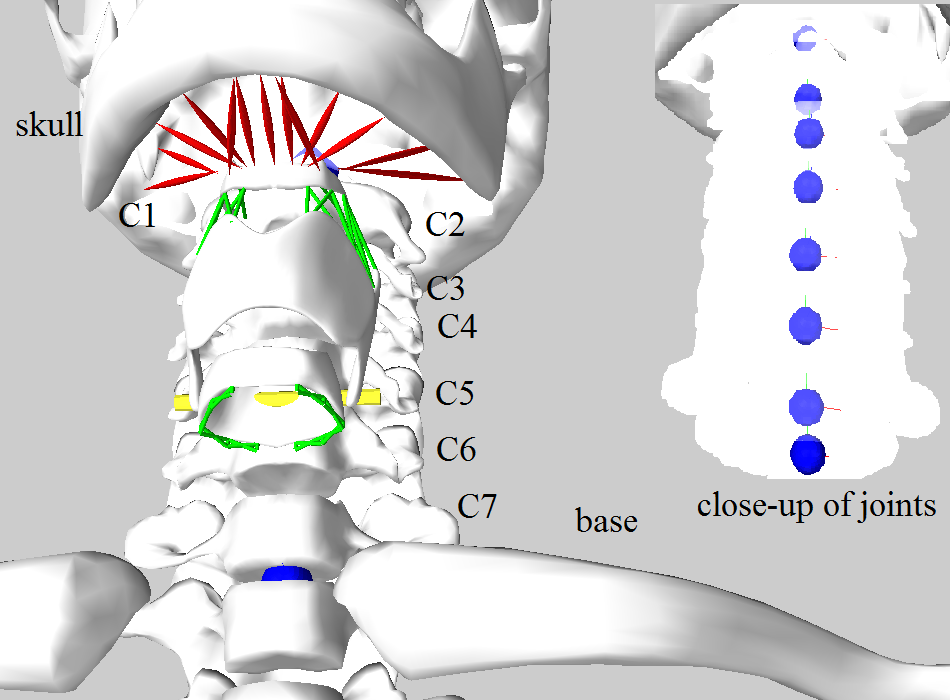
\includegraphics[width=\textwidth]{vriphys/skeletonfinal}
\caption{The neck skeleton where red lines represent muscle actuators, green lines springs, yellow cylinder the revolution joint and blue dots the pivots of the eight cervical joints.}
\label{fig:neckskeleton}
\end{figure}

Since Lee et al.~\cite{Lee:2009:CBM} modeled the upper human body also from the UHM data set, hence we are motivated to use the same mass value assigned to each bone, and the details of the parameters are provided in~\cite{Lee:2008:BMC}. However, unlike their approximation of the inertial properties of the skeleton from the dense volumetric mesh,
%of the surrounding soft tissues by associating inertial parameters of each volumetric element
%to the nearest bone to augment the bone's inertial tensor,
we approximate the inertial parameters of each bone directly from its density $d=m/v$ where $m$ is the mass and $v$ the volume.

%------------------------------------------------------------------------
\subsubsection{\textbf{Muscle Actuator}}
\label{sec:muscleactuationmodel}
We model the muscle actuator as a linearized Hill-type muscle model~\cite{Lee:2006:HUB}. The total muscle force is the sum of the forces from a contractile element (CE) and a parallel element (PE), whereas the length of the tendon is assumed be constant. The CE force is expressed as
\begin{equation}
f_{c}=\alpha f_{o}\mathbf{F}_{l}(l),
\end{equation}
where $0\leq\alpha\leq1$ is the activation level of the muscle, and $f_{o}$ the
maximum force of active muscle. The force-length curve $\mathbf{F}_{l}(l)$ is in the form
\begin{equation}
\mathbf{F}_{l}(l)=\max(0, 0.5(1+\cos(2\pi(\frac{l-l_{o}}{l_{o}})))),
\end{equation}
where $l$ is the length and $l_{o}$ the optimal muscle length at which the maximum isometric force of active muscle is developed. The maximum and minimum at which muscle can produce force is set $0.5l_{o}$ and $1.5l_{o}$, respectively.

The PE force is expressed as
\begin{equation}
f_{p}=\gamma f_{o}\min(\frac{l-l_{o}}{l_{max}-l_{o}},1.0)+d_{m}\dot{e}, l\geq0,
\end{equation}
where $l_{max}$ is the maximum stretched length of the muscle, $d_{m}$ damping coefficient, $\dot{e}$ strain rate, $\gamma$ weighting factor of the passive tension in $f_{m}=f_{c}+f_{p}$.

%-------------------------------------------------------------------------
\subsection{Musculature and Skin Structure}
\label{sec:tissuemodel}
%-------------------------------------------------------------------------
\subsubsection{\textbf{Muscle modeling}}
\label{sec:musclemodeling}
The muscles close to the skin layer are chosen as the relevant underlying soft tissue which are trapezius, sternocleidomastoid, sternohyoid and thyrohyoid. We model them as deformable bodies with volume preservation introducing visual richness of a more detailed 3D muscular model which can facilitate the skin deformation. We use finite element analysis as the convenience in volume conservation. Therefore simulation mesh that is a discrete representation of the muscle volume is generated beforehand based on the geometric data of polygon mesh in the UHM data set.

There are several meshing algorithms~\cite{Labelle:2007:ISF,Molino:2003:acrystalline,Si:2006:quality} handling complex geometry that can be applied. Lee et al.~\cite{Lee:2009:CBM} used Monilo et al.s'~\cite{Molino:2003:acrystalline} method for the meshing of polygon meshes from the UHM data set by first generating a Body-Centered-Cubic tetrahedral lattice completely covering the volume of the human body, and then use an algorithm as~\cite{Sifakis:2007:ACD} to cut this lattice along the skin surface to obtain the volumetric mesh of the human body which resolves the muscle models. However, automatical meshing using the geometric data can produce a large amount of elements, hence make the simulation impractical. Despite we can generate coarser simulation meshes by increasing the element size as shown by Lee et al.s' approach~\cite{Lee:2009:CBM}, refinement will be required to the region especially with high-curvature feature due to higher aspect ratios the elements exhibited and so the large number of simulation elements is still there.

To reduce the number of simulation elements, we do not generate the volumetric meshes using the complete geometric data of the UHM data set. We start by a cleaning step which subjectively select
the geometric data of each muscle polygon mesh as the input to the next step, meshing. Next we will explain how the pipeline is realized.
\begin{figure}
\centering
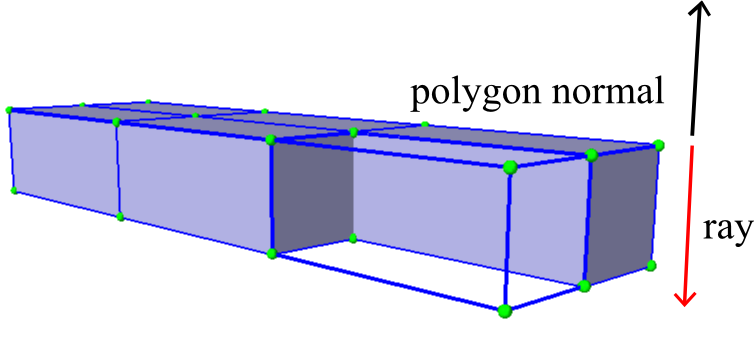
\includegraphics[width=\textwidth]{vriphys/meshing}
\caption{Illustration of the meshing method. The polygon faces are extracted which normals are nearly parallel, ray along the inverse normal direction of each vertex is cast, and then inner node of a hexahedron is defined by picking a point in the 3D line of the ray
according to the parameters (segments and offset).}
\label{fig:meshing}
\end{figure}

Based on an observation of the geometric complexity of the four selected muscles in the UHM data set, we individually take care of each polygon mesh. For sternocleidomastoid, sternohyoid and thyrohyoid particular faces are extracted for which adjacent vertex normals
nearly parallel to each other as regular polygons are distributed on the surface. We cast rays along the inverse normals and take the points as new nodes on the line according the pre-defined offset (2.5 mm) and number of segments (1) (Figure~\ref{fig:meshing}), hence generate 91 hexahedrons for sternocleidomastoid, 90 for sternohyoid and 152 for thyrohyoid. However, this method is not applicable to trapezius due to irregular faces and higher complexity in its geometry. Keeping the effort to reduce the model size, for trapezius, we only extract the neck part because, from an anatomical view, by its FE model the skin patch at the back of the neck is mainly influenced. A tetrahedral mesh generator~\cite{Si:2006:quality} is used, and using a maximum element volume of 1000 $mm^{3}$ and minimum radius-edge ratio of 2.0, the final simulation mesh for trapezius results in 3,497 tetrahedrons.
%\begin{figure}
%\centering
%\includegraphics[width=0.5\textwidth]{images/muscles3}
%\caption{Left: volumetric meshes. Right: their corresponding polygon meshes in UHM data set.}
%\label{fig:muscles}
%\end{figure}

We use the finite simulation method~\cite{Cook:1995:finite} to solve the governing partial differential equations for continuum behavior. On account of the fact that linear elasticity constitutive models are both stable and computationally cheap while a method called \emph{Stiffness Warping} proposed by M\"{u}ller and Gross~\cite{Muller:2004:IVM} can be integrated to handle the displeasing distortion in large rotational deformation, each simulation element is modeled as a co-rotated linear elastic material~\cite{Muller:2004:IVM} instead of a hyperelastic Mooney-Rivlin material as~\cite{Lee:2009:CBM}. It is worth noting that the numerical stabilities of the corotational FEM can be further improved by the approaches proposed by Georgii and Westermann~\cite{Georgii:2008:corotated}.

In our FE models, the solid elements are isoparametric elements associated with a defined local coordinate system, the isometric coordinates. Within an element, the position vector in the global Cartesian coordinate system written as a function of the isoparametric coordinates is the linear interpolation of the spatial coordinates of the element nodes by the element shape functions, and the same parametric interpolation is also used for the displacement field. In our model, we use the shape functions for hexahedral and tetrahedral element defined in FEBio~\cite{Maas:2012:febio}.

Within each element $e$, the deformation map $\Psi$ maps every point $\mbox{\textbf{X}}$ in the undeformed body to point $\mbox{\textbf{x}}=\mbox{\textbf{X}}+\mbox{\textbf{u}}(\mbox{\textbf{X}})$
in the deformed body, and the total strain is obtained by integrating the strain tensor $\mbox{\textbf{F}}=\partial\Psi/\partial\mbox{\textbf{X}}$ at each point over the entire element in the form \begin{equation}
\varepsilon = \frac{1}{2}(\mbox{\textbf{C}}-\mbox{\textbf{I}}),
\end{equation} where $\mbox{\textbf{C}}=\mbox{\textbf{F}}^{T}\mbox{\textbf{F}}$ is the deviatoric Cauchy strain tensor. Given the Young's modulus and Poisson's ratio that are used to form a $\mbox{6}\times\mbox{6}$
matrix $\mbox{\textbf{E}}$, the Cauchy stress tensor is calculated by the equation
\begin{equation}
\sigma = \mbox{\textbf{E}}\cdot\varepsilon.
\end{equation}
The elastic forces $f_{e}$ exerted on the element nodes are derived from the total strain energy and turn out to be linearly dependent on the nodal displacement $\hat{x}=x-x_{0}$ by using the Cauchy strain:
\begin{equation}
f_{e}=-\frac{\partial\varepsilon}{\partial x} = \mbox{\textbf{K}}_{e}\hat{x}
\end{equation}
where $\mbox{\textbf{K}}_{e}$ is the $\mbox{12}\times\mbox{12}$ stiffness matrix of the element and the calculation is described in~\cite{Muller:2002:SRD}.

The artifacts arising from large rotational deformation that happens in neck movements where moment is generated, are removed using the warped stiffness concept on element scale~\cite{Muller:2004:IVM}. The rotated stiffness matrix of an element is calculated by
$\mbox{\textbf{K}}^{'}_{e}=\mbox{\textbf{R}}_{e}\mbox{\textbf{K}}_{e}\mbox{\textbf{R}}^{-1}_{e}$
where the rotational component $\mbox{\textbf{R}}_{e}$ of the element is calculated using the method described in~\cite{Muller:2002:SRD}. Therefore $f_{e}$ is modified as
\begin{equation}
f^{'}_{e}=\mbox{\textbf{K}}^{'}_{e}\hat{x} =
\mbox{\textbf{R}}_{e}\mbox{\textbf{K}}_{e}\mbox{\textbf{R}}^{-1}_{e}x-\mbox{\textbf{R}}_{e}\mbox{\textbf{K}}_{e}x_{0},
\end{equation}
and the whole stiffness matrix $\mbox{\textbf{K}}^{'}$ of the entire mesh is the sum of all element's rotated stiffness matrix.

%-------------------------------------------------------------------------
\subsubsection{\textbf{Integration with Skeleton}}
\label{sec:integration}
In our model, the muscles deform when the skeleton moves. In this section, we begin to describe method to integrate the skeleton with FE models.

A widely used solution consists in constraining any node of the simulation mesh that lies inside or near a bone to a fixed position within the local coordinate frame of that bone. For example the FE
simulation software FEBio~\cite{Maas:2012:febio} provides a tool where we can subjectively select such nodes by area, surface, or volume selection function. Lee et al.~\cite{Lee:2009:CBM} proposed a method to automatically find the nodes to be constrained, and its feasibility lies on the fact that they created one simulation mesh resolving all
tissues except the bones of the human body and the mesh overlaps with the skeleton tightly. Unlike their modeling, we model part of the superficial muscles individually and only some nodes (mainly in the attachment areas where the muscles connect to the bones) of their simulation meshes lie inside or near bones, hence it is difficult to
automatically find these nodes accurately. Finally hence we opt for the selection functions provided by FEBio.

Some parts of the simulation mesh are very close to the skin surface in our model, especially of sternocleidomastoid. It will lead to odd looking patches of the skin if the attached nodes move rigidly with the bones since we will propagate the simulated nodal motion to the skin layer and consequently deform the skin (see Section~\ref{sec:skinmodel}). We address the limitations by implementing the soft constraint concept proposed by Lee et al.~\cite{Lee:2009:CBM}.
\begin{figure}
\begin{center}
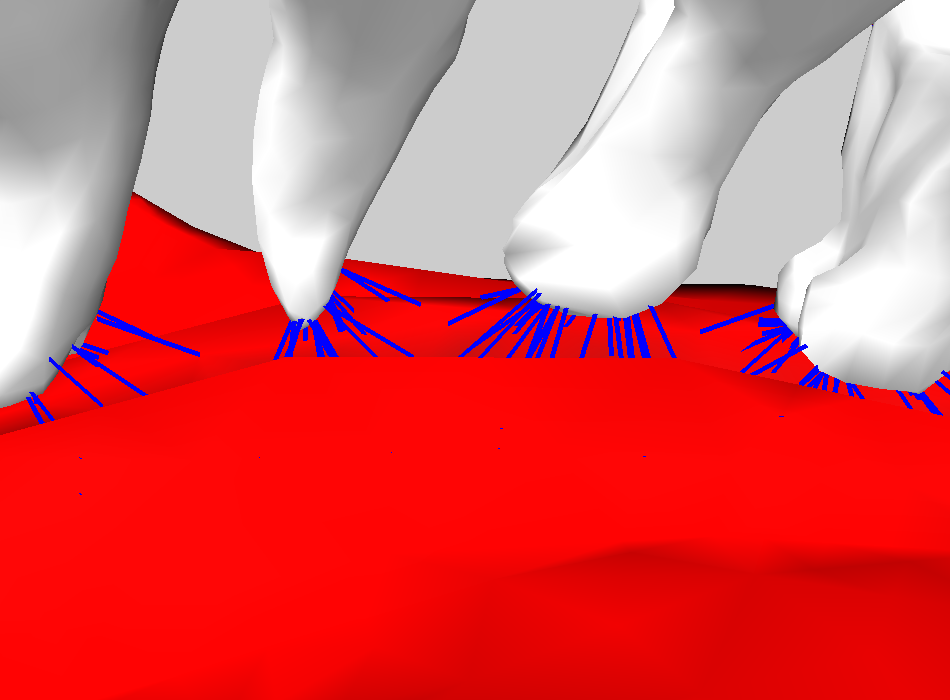
\includegraphics[width=0.45\textwidth]{vriphys/integrationsample}
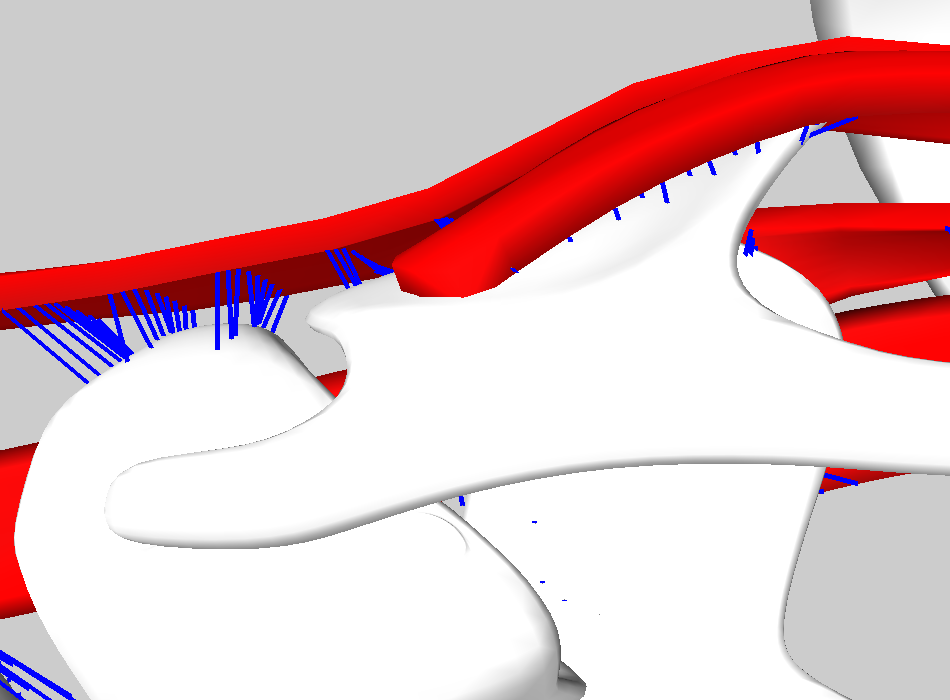
\includegraphics[width=0.45\textwidth]{vriphys/collision}
\caption{\label{fig:integration}
Illustration of the soft constraint on FE models, the blue lines represent constraint springs.}
\end{center}
\end{figure}
We developed an interface to FEBio so the simulation mesh can be imported into its environment. Nodes are selected based on the observation on the anatomy available in the UHM data set. In more details, the nodes which are the closest to the bones underneath are selected. Despite it requires manual labour, in practice, this process is fast and it is tolerable, as a one-time modeling cost. Next we project the node to the surface of the bone by a fast closest point projection method (Section~\ref{sec:skinmodel}) and the projection is attached to the bone. Finally, we connect the node and its projection using an elastic spring which applies traction forces on the node as the bone moves. Figure~\ref{fig:integration} depicts how the FE models are coupled with the bones underneath.

%-------------------------------------------------------------------------
\subsubsection{\textbf{Skin Model}}
\label{sec:skinmodel}
Simulating the dynamic skin deformation based on the simulation of the underlying musculoskeletal model has been investigated. Assassi et al.~\cite{Assassi:2012:dynamic} and Lee et al.~\cite{Lee:2009:CBM} generate the simulation mesh resolving the skin tissue in their lower and upper body, respectively. Nonetheless, the former directly renders the model surface so the visualization largely depends on the element size while the latter barycentrically embeds an high-resolution skin surface as the visualization geometry into the mesh. While it experimentally shows high degree of realism in skin deformation, we cannot afford such simulation considering our performance objective.
\begin{figure}
\begin{center}
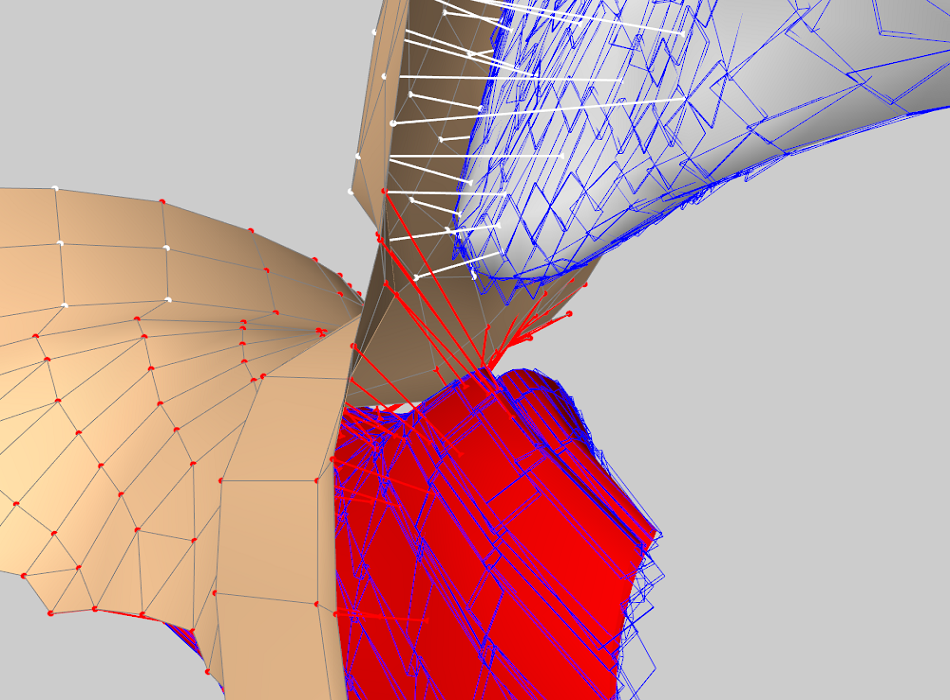
\includegraphics[width=0.45\textwidth]{vriphys/closetpoint2}
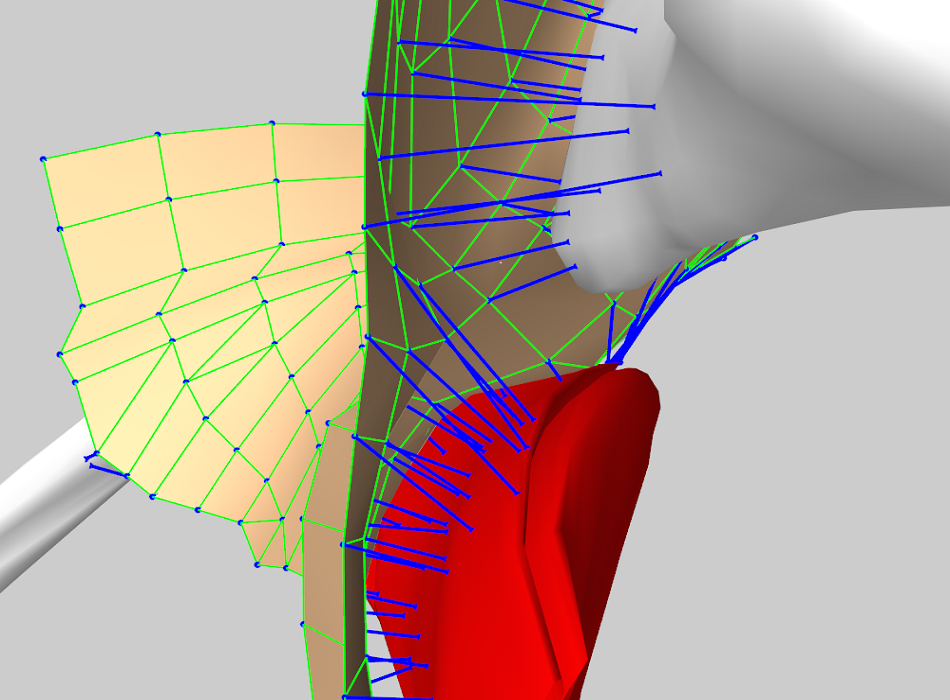
\includegraphics[width=0.45\textwidth]{vriphys/skinmodel2}
\caption{\label{fig:skinmodel}
Illustration of the skin modeling. Left: White and red lines depict the projection maps and blue rectangles are the volume bounding boxes. Right: Blue lines represent connecting springs and green lines the epidermal springs.}
\end{center}
\end{figure}

In the torso model~\cite{Zordan:2004:breathe}, skin simulation is decoupled from the simulation of the underlying model by first recording the trajectories of pre-selected points attached to the model that are the control vertices of a NURBS (Non-uniform rational B-spline) surface. The surface shape is then updated to show skin deformation. The shape of the visualization geometry is implicitly defined by how the control vertices are selected.

We use the mass-spring approach which is popular in real-time simulators like facial animation~\cite{Fratarcangeli:2005:physically,Zhang:2004:NPM}
because it is simple to implement and meets our performance requirements. The human skin is experimentally shown as a multilayered elastic material with non-linear stress-strain relationship based on
the study on the rabbit abdominal skin~\cite{Fratarcangeli:2005:physically}, and the epidermal layer is stiffer than inner layers so its spring stiffness are set to make it moderately resistant to deformation~\cite{Zhang:2004:NPM}.

We use linear spring embedding a damper and the spring force magnitude is a function expressed as
\begin{equation}
f_{s} = k_{s}(l-l_{0})+d_{s}\dot{e},
\label{eq:spring}
\end{equation}
where $k_{s}$, $d{s}$ are elastic and damping coefficients, $l$, $l_{0}$ are its length and slack length, $\dot{e}=\dot{l}/l_{o}$ is the strain rate.

The geometry data of the skin mesh serves as the basis to construct a mass-spring network representing the epidermal layer. We do not model the inner layers yet we use springs as the medium through which the underlying simulated motion is propagated to the upper mass-spring network, and consequently result in the dynamic skin deformation.

From an anatomical view, a patch of the skin surface deforms mainly from the anatomically closest tissue underneath. On account of this fact, the propagation medium should be located between them. To do that, we connect the nodes in the epidermal layer with the points that are attached to the anatomically closest bone or muscle. These points are automatically found based on closest point projection method.

First, to reduce the computation time of finding closest points, we build the oriented bounding box (OBB) trees of the polygon mesh that combines all surface meshes of the underlying bodies using an implementation of the algorithm proposed by Goatishly et al.~\cite{Gottschalk:1996:OHS}. Each skin vertex is projected onto the closest OBB in world coordinates. Secondly, given a skin vertex we decide on which body surface its projection exactly is. We test the projection against each triangulated body surface. If its barycentric coordinate $\left(1- \lambda_{1} - \lambda_{2}\mbox{, }\lambda_{1}\mbox{, }\lambda_{2}\right)$ with respect to a triangle satisfies
$0\leq\lambda_{1}\leq1\mbox{, } 0\leq\lambda_{2}\leq1 \mbox{ and } 0\leq\lambda_{1}+\lambda_{2}\leq1$ then the projection is in this triangle belonging to the body surface. If the body is a FE model, the projection is barycentrically embedded by the nodes of the element containing it, otherwise is attached to the coordinate frame of the rigid body. Finally springs connecting the skin vertices and their
projection are added into the spring network (see Figure~\ref{fig:skinmodel}).
%Our method is more anatomically accurate in contrast to the method of ray casting based on
%the polygon normals, e.g. used in~\cite{fratarcangeli2005}.

%-------------------------------------------------------------------------
\subsection{Numerical Simulation}
\label{sec:numberical}
Let $\mathbf{q}$ be the positions, and $\mathbf{u}$ the velocities of all the dynamical components of the mechanical system, with $\dot{\mathbf{q}}$ related to $\mathbf{u}$ by $\dot{\mathbf{q}} = \mbox{\textbf{Q}}\mathbf{u}$. Let $\mathbf{f}(\mathbf{q}, \mathbf{u}, t)$ be the force produced by all the force effector components,
let $\mbox{\textbf{M}}$ be the (block-diagonal) composite mass matrix. We can ensure that $\mbox{\textbf{M}}$ is constant by representing rigid-body velocity and acceleration in body coordinates. The following governing equation describes the Lagrangian dynamics of the system according to Newton's second law
\begin{equation}
\mbox{\textbf{M}}\mathbf{\dot{u}=f(q,u}, t),
\end{equation}
and it is constrained due to the presence of bilateral (joints and point-surface constraints) and unilateral
constraints (joint limits) in the form
\begin{equation}
\mbox{\textbf{G}}(\mathbf{q})\geq \mathbf{0}, \quad \mbox{\textbf{N}}(\mathbf{q)u} \geq \mathbf{0}.
\end{equation}
For FE simulation, a lumped mass model~\cite{Stavness:2011:CNM} is used to ensure that $\mbox{\textbf{M}}$ is block-diagonal.

As the presence of the FE models, the system is stiff and therefore we need an implicity time integrator for efficient performance. We opt for the simulation framework of Stavness et al.~\cite{Stavness:2011:CNM},
where the Newmark integrator with $\lambda=\frac{1}{2}$ and $\beta=\frac{1}{4}$ is used and hence the step-based updating rule is formulated as a mixed linear complementarity problem which is solved by Pardiso solver\cite{Schenk:2004:solving}.

%-------------------------------------------------------------------------
\section{Experiments}
\label{sec:experiments}
In the experiments, we use the parameters of the muscle actuators (maximum muscle forces) and crossed springs (stiffness) from~\cite{Stavness:2011:CNM}. The FE models have a Young's modulus of 50 MPa and a Poisson's ratio of 0.4. We set stiffness to 1.2$\times 10^{3}N\cdot m^{-1}$ to epidermal springs, connecting springs to 0.5 $\times10^{3}N\cdot m^{-1}$, and constraint springs to 2.0 $\times10^{3}N\cdot m^{-1}$. All simulations are run on a laptop with an Intel Core i7 2.4Ghz processor and 6 GB memory.

The head movements mainly include flexion, extension, rotation and lateral flexion. They are:
\begin{itemize}
\item \textbf{Flexion}: moving the head forward at the joint just below the skull.
\item \textbf{Extension}: moving the head backward at the joint just below the skull.
\item \textbf{Rotation}: turning the head to the side (right or left) at a joint below the skull.
\item \textbf{Lateral flexion}: moving the head toward the shoulder (left or right) at a joint below the skull.
\end{itemize}
In facial animation, a notable visualization is the neck skin deforms when the jaw opens. Therefore, to show the level of realism of the neck animation our model can offer, we demonstrate the result of the four head movements and the jaw openning.

We extract the frames under extreme postures for each testing movements from the simulation video of the musculoskeletal system and present as shown in Figure~\ref{fig:musclesim}.
\begin{figure}
\begin{center}
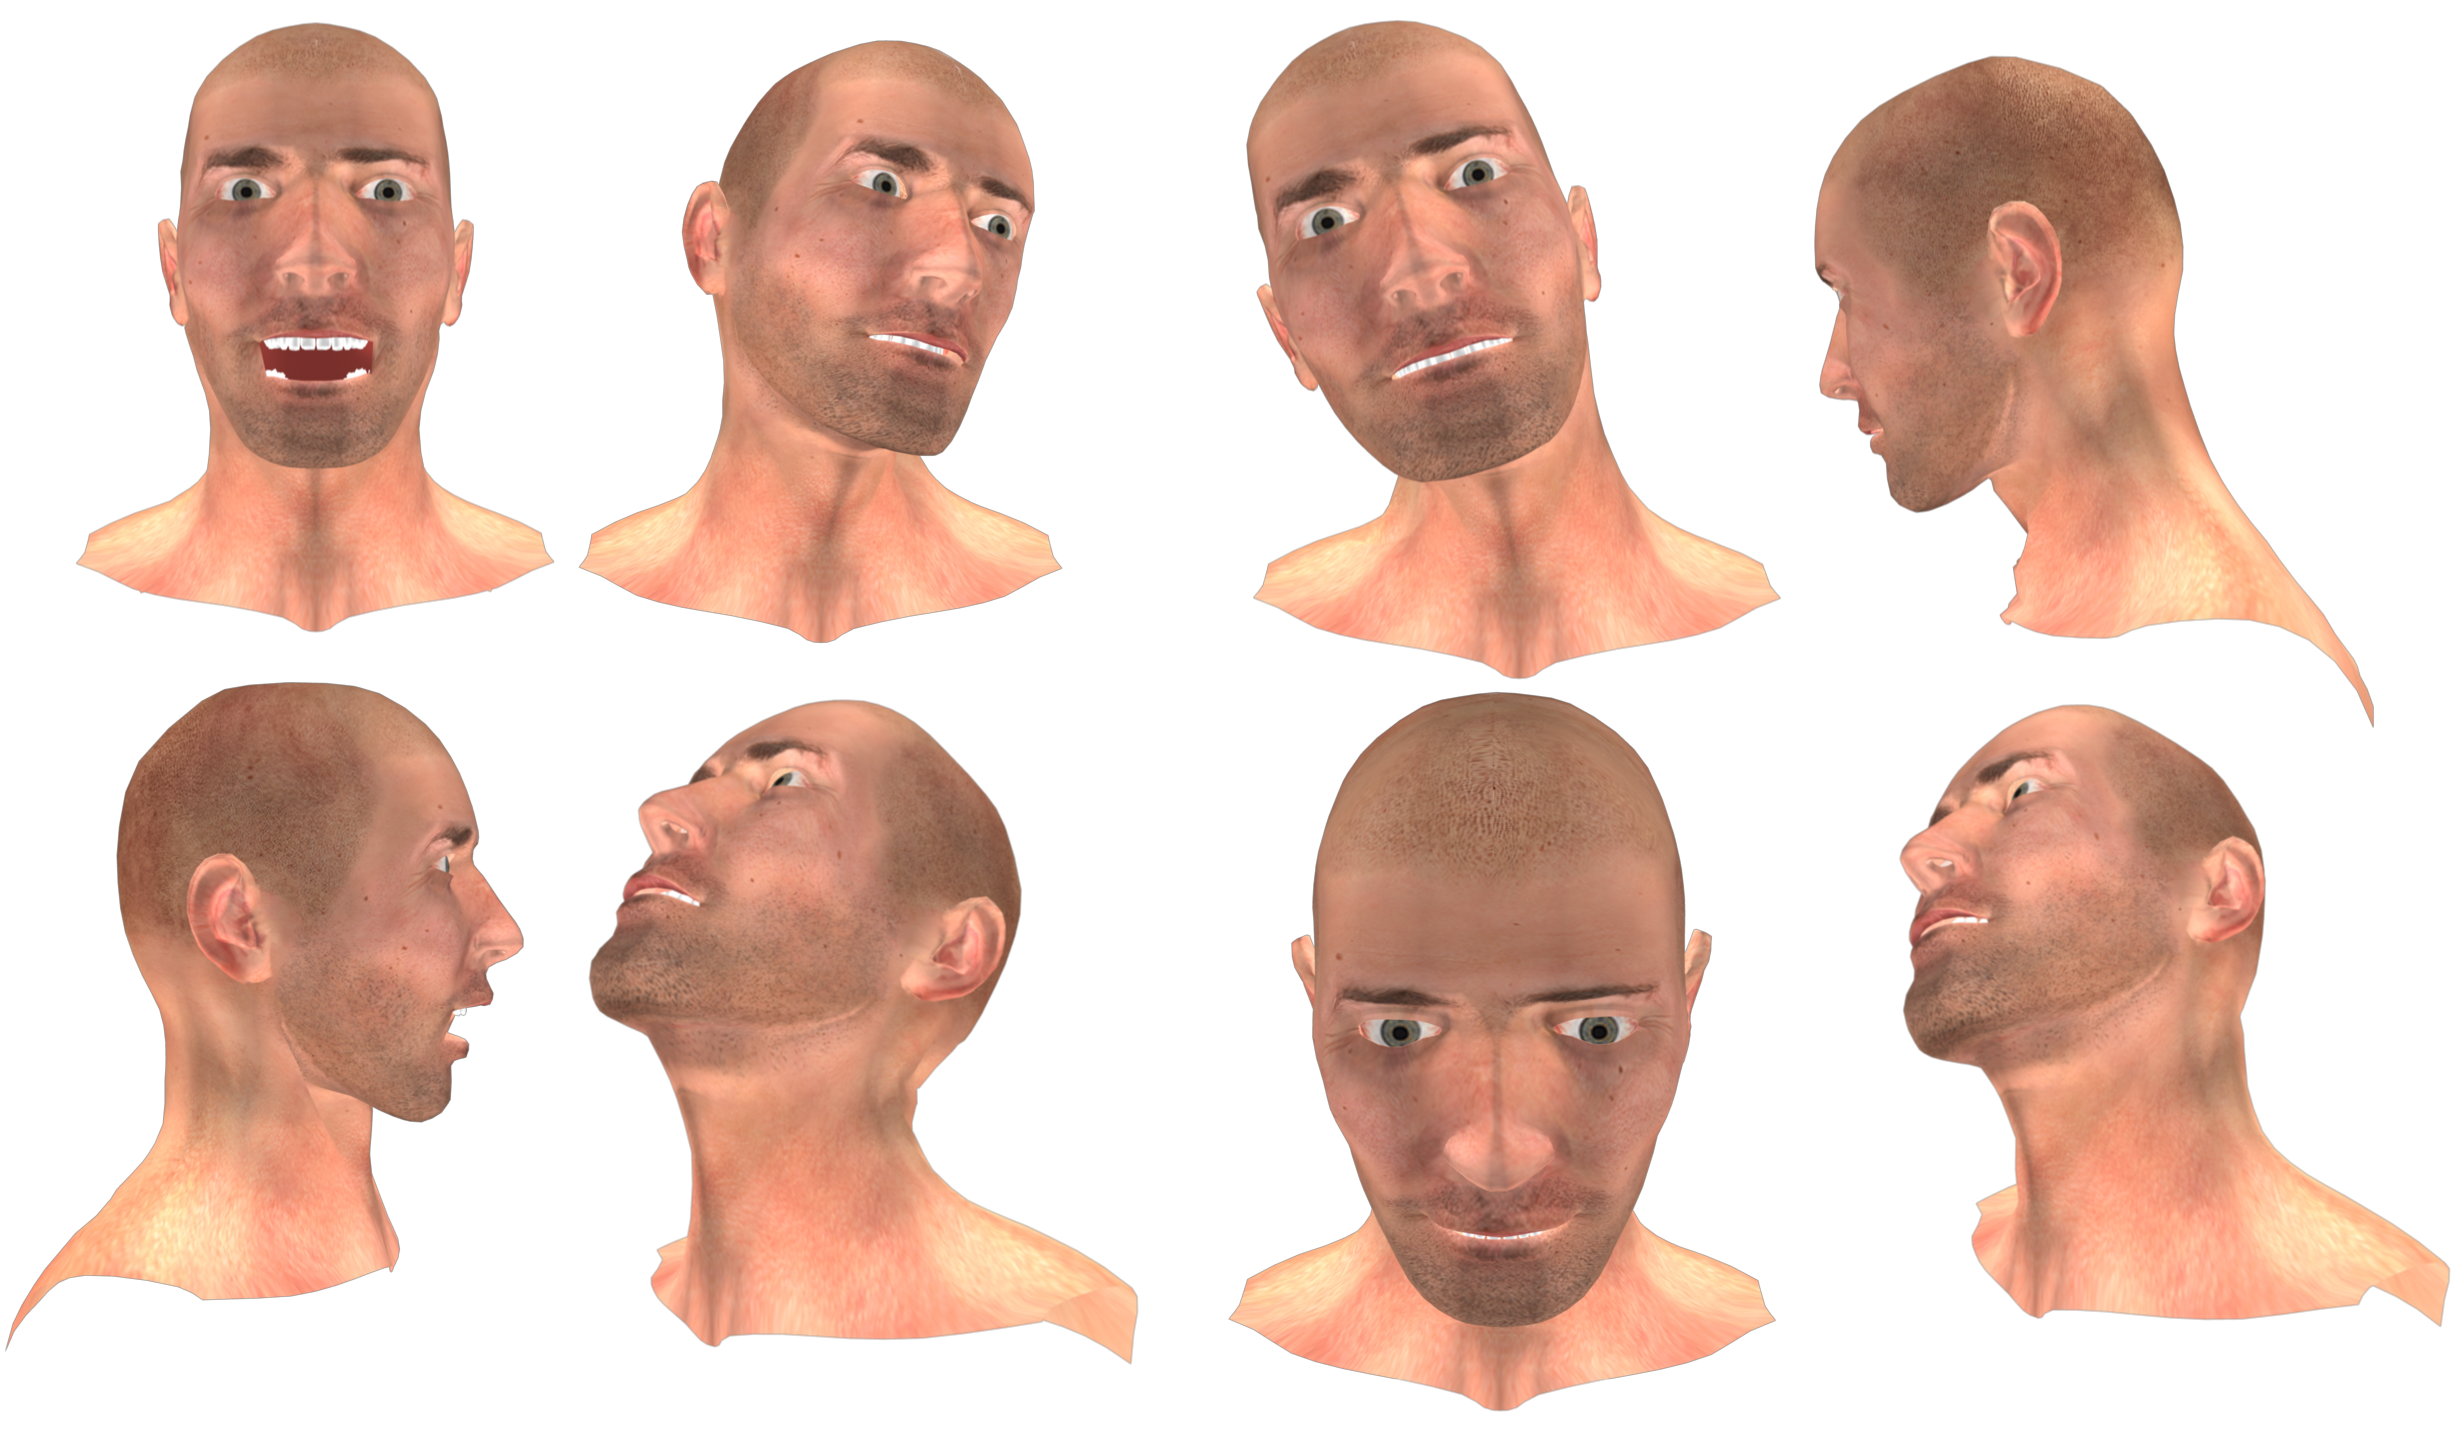
\includegraphics[width=\textwidth]{vriphys/final}
\caption{Some frames of animation we generated using the simulation results of our physical neck model which is from biomechanical modeling.}
\label{fig:final}
\end{center}
\end{figure}

A comparison with the popular technique, namely the linear blend skinning, is conducted. We compare the animation at a pose, and by referring to a static photo of a human neck at the same pose, to show that the simulation deliver more accurate results. The comparison is shown in Figure~\ref{fig:compare}. Muscles in our model are modeled symmetrically from the left and right, therefore we only show the simulation frames of one-side rotation and lateral flexion.

Our model based on biomechanical modeling also can reproduce a wide range of lifelike animation. It is interesting to play the model by exciting the muscle actuators and rotate any cervical joints, while realistic animation is generated. We show some frames from the simulation video in Figure~\ref{fig:final}.

Recall that, for performance issue, we do not model all superficial muscles available in the UHM data set, therefore the simulated musculoskeletal dynamics is not complete enough to conform with the real neck animation while can guarantee the high-fidelity emulation (as shown in Figure~\ref{fig:compare}). We also bind the vertices to underlying bodies according to the anatomy we incorporated, hence the less anatomy we use, the less accurate the vertex binding is.

Modeling more even all anatomical structures, or a nonlinear multilayered skin modeling like~\cite{Zhang:2004:NPM,Fratarcangeli:2005:physically} will definitely increase the memory consumption in order to store the states during the simulation. Additional constraints (attaching proper finite nodes to bones) would be required and therefore would increase the size of influenced matrices in the numerical simulation, hence resulting in higher time complexity. Based on these facts, we trade the speed for accuracy, yet as shown in the figures and accompanying video, our model still offers realistic animation.

%-------------------------------------------------------------------------
\section{Discussion}
\label{sec:dis}
We presented a physically-based model of the human neck. The simulations were performed at interactive rates (average 20 FPS) and results showed the realism the model can deliver. Considering the computational cost, we only modeled the most relevant anatomical structures available in a 3D digital model and form a Lagrangian dynamic system which is solved by a semi-implicity time integrator.

Our model experimentally demonstrated that physically-based modeling can produce skin deformation reflecting the muscular and dynamic effects, and showed that the linear elasticity constitutive models are both stable and computationally cheap, therefore is suitable for soft tissue simulation in neck animation. Our method of skin modeling highlights in automatically binding of skin vertices to underlying
muscles and bones via linear elastic springs in an anatomical manner, and it is quite easy to implement and fast to simulate.

In current model, the muscle actuators are only used for the interconnection between jaw and hyoid, we plan to implement the muscle actuation model using them so that the simulation of the muscle tensioning can be achieved which is difficult to skeleton-driven method, especially arising from strong emotional expression in the face. We also plan to compare our method with methods of capturing real humans, to investigate the applicability of our model in character animation.
\begin{figure}
\begin{center}
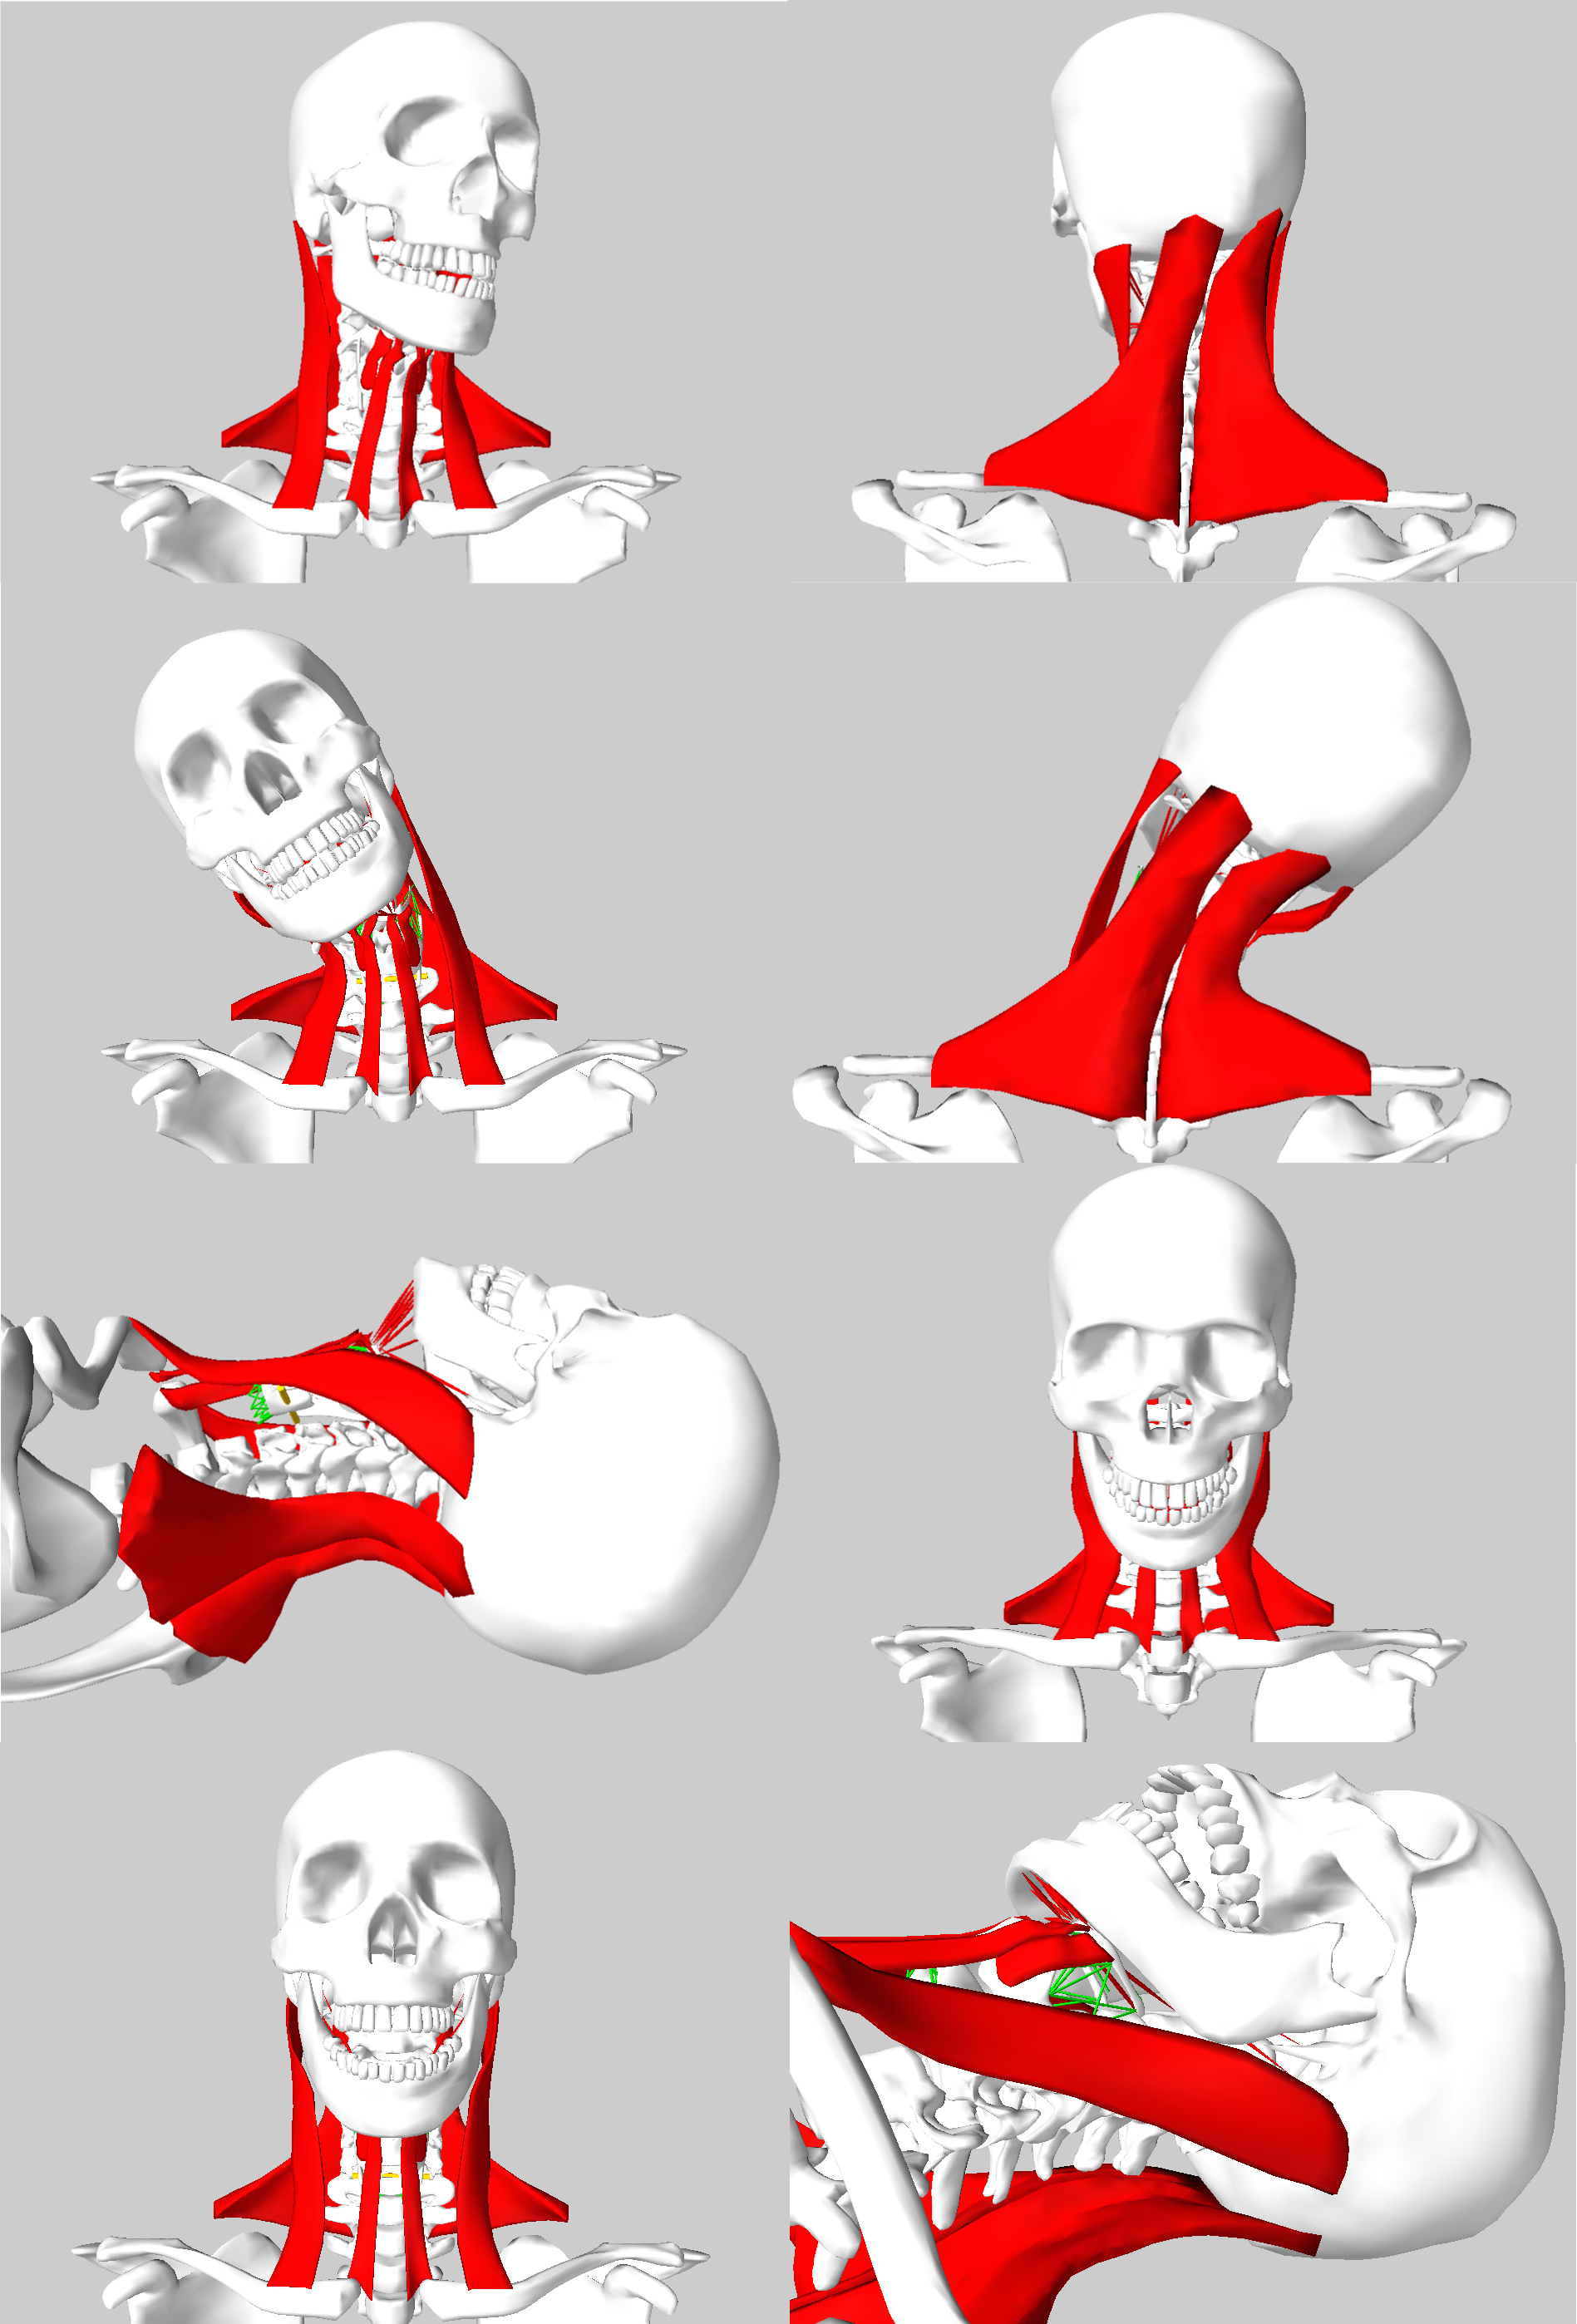
\includegraphics[width=\textwidth]{vriphys/musclesim}
\caption{Frames from the simulation of the underlying components (muscles, skeleton, actuators and springs).}
\label{fig:musclesim}
\end{center}
\end{figure}
\begin{figure}
\begin{center}
\includegraphics[width=\textwidth]{vriphys/compare}
\caption{Referring to the corresponding static photos, linear blend skinning exhibits artifacts and cannot generate muscular and dynamic effects reflected in the skin, while our model simulates lifelike
head poses and neck skin deformation where the visible muscle motion is reflected.}
\label{fig:compare}
\end{center}
\end{figure}
